Il se dégage des objectifs le besoin de présenter à l'utilisateur les solutions du casse-tête et de lui permettre d'interagir intuitivement avec l'application. Afin de répondre à ce besoin, il est nécessaire d'avoir un affichage volumétrique (3D) et une interface permettant la lecture des entrées des périphériques courants (clavier, souris). Nous avons donc décidé d'utiliser OpenGL (Open Graphics Library) comme librairie graphique et GLFW (GL FrameWork) comme librairie de gestion de fenêtre et d'entrées.

Afin de permettre des calculs asynchrones à la représentation graphique du cube serpent, nous avons décidé de créer un thread dédié à cette représentation qui aurait pour but la simple lecture de données relatives au casse tête. En limitant la fréquence de rafraichissement de l'affichage à 60 images/secondes, le temps processeur est épargné de manière à favoriser les calculs relatifs à la résolution,  la fluidité d'affichage est garantie, et les conflits de lecture deviennent très peu fréquents (et même imperceptibles).

\section{OpenGL}

OpenGL (Open Graphics Library) est un ensemble normalisé de fonctions de calcul d'images 2D ou 3D lancé par Silicon Graphics en 1992. Cette interface de programmation est disponible sur de nombreuses plateformes où elle est utilisée pour des applications qui vont du jeu vidéo jusqu'à la CAO en passant par la modélisation.

\begin{quotation}
 OpenGL permet à un programme de déclarer la géométrie d'objets sous forme de points, de vecteurs, de polygones, de bitmaps et de textures. OpenGL effectue ensuite des calculs de projection en vue de déterminer l'image à l'écran, en tenant compte de la distance, de l'orientation, des ombres, de la transparence et du cadrage.\newline
 [source: http://fr.wikipedia.org/wiki/OpenGL]
\end{quotation}

Nous avons choisi de restreindre notre code à la version 2.1 d'OpenGL pour des raisons de compatibilité, celle-ci étant supportée par tous les pilotes de carte graphique récents. Cette version apporte le concept de pipeline programmable: certaines parties de la création d'image sont codées par le développeur, compilées et exécutées par le GPU. Ces programmes sont appelés shaders et permettent un contrôle accru du procédé de calcul d'image.

\begin{figure}[h]
 \centering
 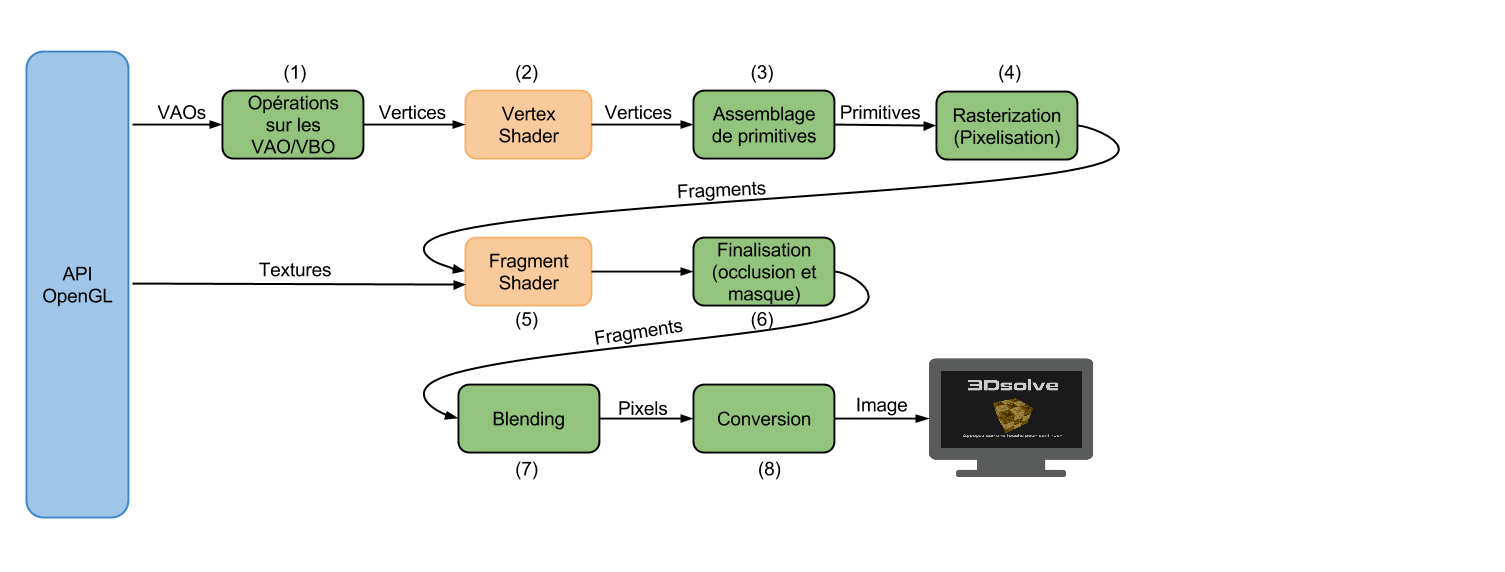
\includegraphics[scale=0.3,keepaspectratio=true]{img/pipeline.png}
 \caption{Le pipeline programmable (simplifié)}
 \label{pipeline}
\end{figure}

Les données (Vertices, UV, textures) et les shaders sont tous chargés dans la mémoire graphique au démarrage du programme, permettant ainsi de réduire grandement le flux de données sur le bus graphique. Ainsi, seuls des identifiants (entiers) sont à communiquer au GPU pour choisir sur quelles données sont exécutées les opérations.
    La figure~\ref{pipeline} détaille les différentes étapes clés du calcul d'une image au sein de la carte graphique:

\begin{enumerate}
 \item Dans le programme, on informe le GPU d'utiliser un VAO (Vertex Array Object), qui va contenir des informations relatives aux vertices (points dans l'espace). Dans notre cas, un VAO contient un tableau de vertices (x, y, z) et un tableau de coordonnées de texture (U, V) pour chaque vertex (ces tableaux sont appelés VBO, Vertex Buffer Object). Cet objet est traité en (1) et execute l'instruction suivante pour chaque vertex du VAO.
 \item Ces vertices sont ensuite traités par le /vertex shader/ (2) (détaillé par la suite), qui effectue des opérations de calcul vectoriel.
 \item Une fois transformés, ces vertices sont assemblés en (3) pour former des primitives. Dans notre cas, une primitive est un triangle, formé par un triplet de vertices adjacents dans le premier tableau du VAO.
 \item Vient ensuite l'étape de rasterization (4): des fragments de pixels sont créés à partir des primitives. Un fragment correspond à une subdivision surfacique de primitive de la taille d'un échantillon de pixel, c'est une conversion d'une information vectorielle vers une information échantillonnée.
 \item Les fragments ainsi créés sont ensuite traités par le /fragment shader/ (5) (détaillé par la suite), qui va "coller" la texture renseignée par le programme sur le fragment en fonction de sa position sur la primitive.
 \item Les fragments ayant les mêmes coordonnées à l'écran sont ensuite ordonnés en fonction de la position de la primitive dont il est issu: un fragment issu d'une primitive cachée par une autre sera placé "derrière" celui issu de la primitive le cachant, quel que soit l'ordre dans lesquels ils ont été traités préalablement (6). Les primitives en arrière plan seront donc partiellement ou totalement occultées.
 \item Ces fragments ordonnées sont ensuite fusionnés en pixels (7). Cette étape réalise deux opérations majoritaires: la fusion de couleur des fragments (en fonction de leur transparence) en échantillons, et le rassemblement de ces échantillons pour former un pixel. L’intérêt de posséder plusieurs échantillons est entre autres l'anti-crénelage (lissage des traits). On peut dire qu'un pixel est issu de n fragments, avec n = nombre d'échantillons * nombre de primitives sous le pixel.
 \item Ces pixels sont ensuite convertis dans le format d'image spécifié par l'application, ici déterminé par le système d'exploitation, puis affichés à  l'écran.
\end{enumerate}

\section{Données}
Les données contenues dans les VAO et les textures sont issues de fichiers afin de faciliter leur création et leur modification. On peut trouver les modèles 3D dans le dossier "stc" et les textures dans le dossier "textures".

Nous avons adopté deux formats de modèles 3D différents au cours du développement, STC (format propre) et le format OBJ de WaveFront (très courant grâce à sa simplicité de codage). Le format STC décrit les données telles qu'elles seront agencées dans les VAOs tandis que le format OBJ est plus complexe, mais globalement plus pratique. Il contient une suite de vertices (préfixe "v"), de vecteurs normaux (préfixe "vn"), de coordonnées de texture (préfixe "vt") et des descripteurs de primitives (préfixe "f") associant pour chaque primitive trois triplets (vertex/normale/coordonnée de texture). Une fois décodées, ces données sont transférées dans la mémoire graphique par les VAOs.

Pour les textures, nous avons choisi d'utiliser le format PNG, pour sa compression sans perte, son canal de transparence et son format largement documenté. La bibliothèque lodePNG a été utilisée pour décoder ces textures de manière simple. Une fois décodées, elles sont transférées dans la mémoire graphique par des "texture buffers".

\section{Utilisation des données}
Les vertices des VAO ne contiennent que des coordonnées relatives au centre de l'objet, il est donc nécessaire de les transformer dans l'espace afin de les déplacer, de les faire tourner et de changer leur échelle. Ces opérations sont réalisées au travers de calcul matriciel à l'intérieur du /vertex shader/. En effet, les GPU sont optimisés afin de réaliser de nombreuses multiplications matricielles à la chaîne. Voici une partie du code de notre vertex shader principal:\newline

\verb|gl_Position = VP * W * vec4 (vertex_position, 1.0);|\newline

Dans ce code on renseigne au GPU la nouvelle position de notre vertex, multiplié par deux matrices. La première, VP (View-Projection) correspond à la matrice de projection de l'espace en trois dimensions vers un espace en deux dimensions (Calculée à partir de la caméra) et la deuxième, W (World position) correspond à  la position de l'objet dont est issu le vertex dans cet espace en trois dimensions.

Ces matrices ne sont modifiés qu'une fois par image (alors que tous les vertices sont calculés à chaque image), il est donc judicieux de les calculer par le CPU et de les envoyer via le bus graphique. La matrice VP est calculée en fonction de la caméra, qui est modifiée par les actions de l'utilisateur. La matrice W est calculée par rapport à la position d'un cube dans notre espace en trois dimension virtuel.

Le fragment shader quant à lui permet de "coller" une partie de texture préalablement choisie sur un fragment. Cette opération est effectuée grâce aux coordonnées de texture (UV): elles permettent de relier un vertex (x, y, z) à un point d'une texture (u, v), ce qui permet de déformer la texture en déformant la primitive associée.

\begin{figure}[h]
 \centering
 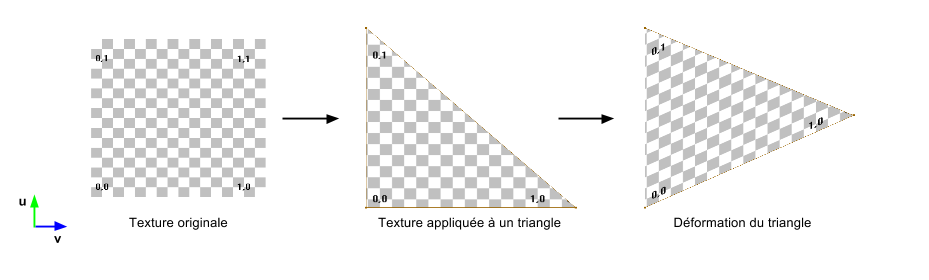
\includegraphics[scale=0.4,keepaspectratio=true]{img/uvexpl.png}
 \caption{Explication UV}
 \label{uv}
\end{figure}

Voici une partie du code de notre fragment shader principal:\newline

\verb|gl_FragColor = vec4(texture2D( CurTex, UV ).rgb, alpha);|\newline

Dans ce code, on renseigne au GPU d'aller chercher une portion de texture à la coordonnée (u, v), de lui ajouter une valeur de transparence arbitraire définie dans notre programme et de l'associer au fragment traité.
